\documentclass[UTF8,11pt]{report}

\usepackage{xeCJK}

\usepackage{amsmath}
\usepackage{url}
\usepackage[colorlinks,linkcolor=black,anchorcolor=black,citecolor=black,urlcolor=black]{hyperref}
\renewcommand\thesection{\arabic{section}}

\usepackage{graphicx}
\usepackage{booktabs}
\usepackage{cite}

\title{VLSI供电网络静态分析算法设计报告}
\author{计62 杜政晓 2016011014}
\begin{document}
\maketitle
\section{Introduction}
常见的数字电路都是由各种各样的门电路组成的. 每个门都有输入管脚和输出管脚. 但是我们经常忽略的是, 门电路还需要连接到电源和地才能工作, 也就是还有$V_{dd}$和$V_{cc}$管脚. 

在电路布局的时候,理论上我们只需要将这些管脚通过线路连接到板子上的电源和地. 但是不幸的是, 真实世界中的导线上总是存在着电阻. 当导线中有电流流过的时候, 电阻就会消耗一部分电压. 这些因素的存在使得门电路的电源和地管脚上的电压并不严格等于理想的电源和地的电压.

\begin{figure}[!ht]
	\centering
	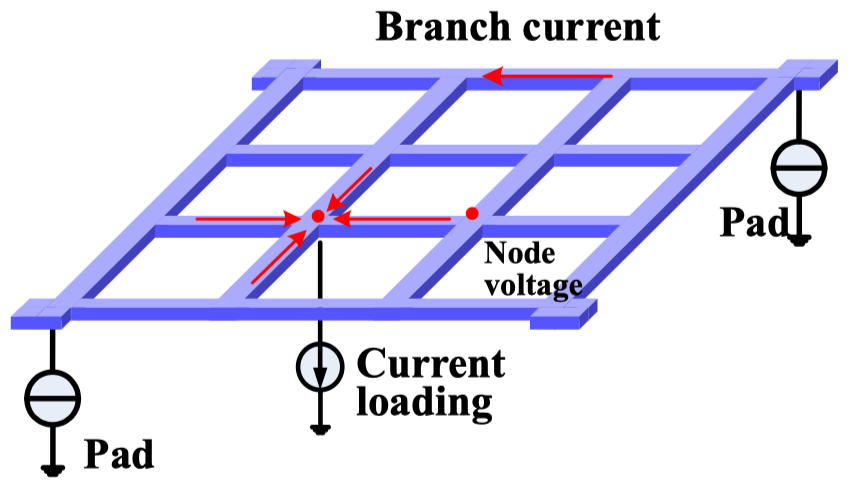
\includegraphics[width=0.7\textwidth]{circuit}
\end{figure}

对于门电路来说, 如果电源和地的电压不符合要求, 会导致门电路的性能表现不符合预期, 比如延迟时间, 建立时间变长. 这就很有可能导致电路的时序出现问题.

因此, 为了电路运行的可靠性, 除了正常的时序分析之外, 在布线完成之后还需要进行供电网络的分析, 检查各个门电路供电管脚的电压是否符合要求, 实际电压与理想电压之间的差距是否会威胁到电路的正常工作. 其中核心的一步, 就是求解出各个门电路供电管脚处的电压. 因为这一分析是在计算$\Delta V = IR$, 所以也称为IR Drop分析.

IR drop分析可以分为两类: 静态分析与动态分析. 静态分析考虑的是电路处于稳态的情况。 这种情况下只需要考虑各导线上的电阻的影响. 而动态分析考虑的是电路在电路处于稳态的建立过程中的情况, 这种情况下门电路本身处于状态转换中, 因此在电源和地管脚之间会有电流流过, 使得电路可能在瞬间通过很大的电流, 使得IR drop非常明显. 按照课程要求, 我们实现的是静态的IR drop分析。

我们的贡献为:实现了一个大规模的静态供电网络分析工具PowerGrid Solver,并在不同规模的测试样例上做了性能测试,与当前普遍使用的开源库相比,表现出了明显的性能优势。
\section{Preliminary}
\subsection{理论分析}
\label{subsec:theory}
一个电路可以看做是有$N$个节点, $M$条边的图. 其关联矩阵为$\mathbf{A}$。
设各个节点上的电压为向量$\vec{u}$, 各条边上的电流为向量$\vec{i}$, 则根据基尔霍夫电流定律, 有
\begin{equation}
	\mathbf{A}^Ti=I
\end{equation}
其中$I$由与节点相连的电流源决定. 根据欧姆定律, 有
\begin{equation}
	i=\mathbf{G}(U-\mathbf{A}u)
\end{equation}
其中$U$由边上的电压源决定. 用两个方程消去$i$得到
\begin{equation}
	\mathbf{A}^T\mathbf{G}\mathbf{A}u=\mathbf{A}^T\mathbf{G}U-I
\end{equation}
因此我们只需要求解这个线性方程组,就可以得到供电网络上各节点上的电压。
\subsection{输入输出格式}
我们选择的输入文件格式为SPICE netlist,一是因为实验所用的数据集使用的是该格式,二是便于与工业界广泛使用的SPICE软件兼容。SPICE netlist是一种面向元件的电路描述方式,除去层和线网的划分外,其中的每一行代表了电路中的一个元件(在静态分析中,可能出现的只有电阻,导线,电压源和电流源)。
\section{Approach}
\subsection{数据预处理}
数据预处理的第一步是将数据读入。程序会依次解析输入文件的每一行,获取到元件和节点的位置关系(电流源、电压源、电阻都是在两个节点之间的)。

然后程序会将阻值为0或者是小于某个常数(我们这里取的是1e-5)的电阻视作短路,将短路的节点合并为一个节点。这一步对于后续的求解非常重要,因为短路的边电导非常大,会导致线性方程组的系数矩阵的条件数非常大,求解的数值稳定性较差。

然后结合这个问题的性质,我们可以发现整个电路可以分成和电源相连的电路与和地相连的电路,而且这两个电路不会有连接。所以我们可以将整个电路的求解分成两个较小规模的电路求解,因为线性方程组的求解复杂度一般是超线性的,所以分解也可以加快求解的速度。

最后,程序根据化简分解后的两个电路生成生成两个\ref{subsec:theory}中描述的线性方程组。显然这里的方程组是一个非常稀疏的矩阵(原因在于A是稀疏的),因此我们使用了稀疏矩阵中常用的三元组法来存储,只需要存储非0的项,比用二维数组存储每一项要节省空间。
\subsection{求解算法}
经过预处理之后,问题就转化为了两个大规模稀疏线性方程组的求解。我们实现的线性方程组的求解方法可以分成两类,一类是直接解法,一类是迭代法。直接解法包括高斯消元法。迭代法包括Jacobi迭代,Gauss-Seidel迭代法,超松弛迭代法和共轭梯度法。
\subsubsection{(选主元的)高斯消元法}
高斯消元法每个人在线性代数中都很熟悉。就是通过对第$i+1$到第$n$行加上第$i$行的倍数,来将第$i$个元素消为0。这样得到的就是一个上三角矩阵,可以直接从最后一行开始用回代法求解。

选主元的高斯消元法是对高斯消元法的一个改进,因为高斯消元的时候,如果第$i$行的第$i$个元素绝对值非常小的话,其他行就要减去第$i$行一个较大的倍数。为了避免这一情况,当我们要消去第$i$列的时候,首先从第$i$到$n$行选出第$i$个元素绝对值最大的行,与第$i$行交换位置。
\subsubsection{Jacobi迭代法}
所有的迭代法的基本思路都是一样的,就是找到线性方程组的解满足的某个恒等式$x=Bx+f$,然后从某个随机的$x^{(0)}$开始,迭代求$x^{(k+1)}=Bx^{(k)}+f$,直到前后两次迭代结果的差别小于误差限。

Jacobi迭代的公式为:
\begin{equation}
	x_i^{(k+1)}=-\frac{1}{a_{ii}}\sum_{j\neq i}{a_{ij}}x_j^{(k)}+\frac{b_i}{a_{ii}}
\end{equation}
\subsubsection{Gauss-Seidel迭代法}
Gauss-Seidel迭代的公式和Jacobi迭代很相似
\begin{equation}
	x_i^{(k+1)}=-\frac{1}{a_{ii}}\sum_{j=1}^{i-1}{a_{ij}}x_j^{(k+1)}-\frac{1}{a_{ii}}\sum_{j=i+1}^{n}{a_{ij}}x_j^{(k)}+\frac{b_i}{a_{ii}}
\end{equation}
\subsubsection{超松弛迭代法}
超松弛迭代可以看做是一般化的Gauss-Seidel迭代
\begin{equation}
	x_i^{(k+1)}=(1-\omega)x_i^{(k)}+\frac{\omega}{a_{ii}}(b_i-\sum_{j=1}^{i-1}{a_{ij}}x_j^{(k+1)}-\sum_{j=i+1}^{n}{a_{ij}}x_j^{(k)})	
\end{equation}
其中$\omega$称为迭代因子,对于求解的收敛性和速度有很大的影响。
\subsubsection{共轭梯度法}
共轭梯度法是迭代法中最复杂的一种,但一般也是收敛速度最快的一种。而且有多种方法可以加速收敛,所以经常在实际中用来求解线性方程组,尤其是系数矩阵为稀疏矩阵的情况。
\begin{align}
	\alpha_k=\frac{(r^{(k)},r^{(k)})}{(P^{(k)},AP^{(k)})}\\
	x^{(k+1)}=x^{(k)}+\alpha_kP^{(k)}\\
	r^{(k+1)}=r^{(k)}-\alpha_k AP^{(k)}\\
	\beta_k=\frac{(r^{(k+1)}, r^{(k+1)})}{(r^{(k)}, r^{(k)})}\\
	P^{(k+1)}=r^{(k+1)}+\beta_k P^{(k)}
\end{align}
	\subsubsection{收敛性分析}
我们要求解的线性方程组的系数矩阵为$A^TGA$,可以证明这是一个严格对角占优矩阵。因此对于Jacobi迭代法、Gauss-Seidel迭代法来说是可以保证收敛的。同时对于$0<\omega<2$,超松弛迭也是可以保证收敛的。
\subsubsection{复杂度分析}
使用高斯消元法直接求解的复杂度为$O(N^3)$,对于大规模矩阵来说,这一复杂度几乎是不可接受的。

迭代法的复杂度为$O(kM)$,$k$为迭代次数,而$M$为图的边数。对于稀疏图产生的稀疏矩阵来说,$M=O(N)$,因此迭代法经常用于稀疏的线性方程组的求解。而让迭代法更快的关键就在于加快迭代的收敛速度,从而减少迭代次数。
\subsection{求解加速}
\subsubsection{利用预条件子加快收敛}
预条件子是线性方程组求解中常用的一种技巧。在求解线性方程组$\mathbf{A}x=b$时, 通过预条件子$\mathbf{P}$转化为条件数更小的方程$\mathbf{P}^{-1}\mathbf{A}x=\mathbf{P}^{-1}b$,从而使得迭代的收敛速度更快。使用了预条件子处理的共轭梯度法就称为预条件的共轭梯度法(Preconditioned Conjugate Gradient Method)。

一个矩阵的预条件子有很多种求法。实际中常用的是不完全的Cholesky分解。但是因为我们的系数矩阵是严格对角占优矩阵,所以$\mathbf{P}$可以简单取做A的对角矩阵, 即$P^{-1}_{ij} = \frac{\delta_{ij}}{A_{ij}}$。
\subsubsection{利用多线程加速矩阵运算}
在共轭梯度法的求解中,绝大部分操作都是$O(N)$的,只有一个矩阵和向量相乘$\mathbf{A}\cdot{P}$是$O(N^2)$的,占据了求解的大部分时间。因为矩阵和向量相乘的时候,各行之间是无关的,所以可以并行。我们使用了OpenMP来实现多线程的矩阵乘法。在四核CPU的机器上加速比可以达到2.0以上。
\section{Experiment}
\subsection{实验设定}
\subsubsection{数据集}
我们使用的数据集是IBM Power Grid Benchmarks\cite{4483978},一个静态供电网络分析中经常使用的benchmark。不同benchmark的规模对比见表\ref{tab:dataset}。
\begin{figure}[!ht]
	\centering
	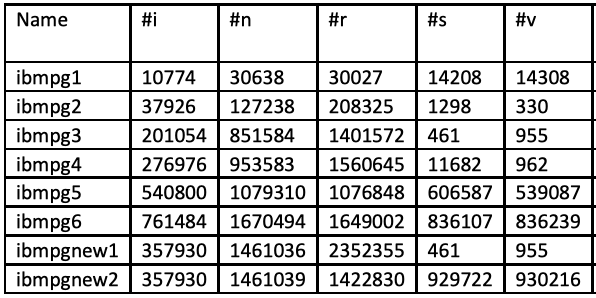
\includegraphics[width=0.8\textwidth]{dataset}
	\caption{IBM Power Grid Benchmark规模}
	\label{tab:dataset}
\end{figure}

可以看出,这个benchmark的规模虽然和工业界中几亿的节点数还有差距,但是作为在个人电脑上进行测试还是很合适的。

\subsubsection{实验环境}
实验时使用的电脑是我个人的电脑,MacBook Pro 2018, 处理器2.3 GHz Intel Core i5(四核),内存8 GB 2133 MHz LPDDR3。

\subsection{结果}
首先,我们对比了不同的线性方程组求解算法的性能。结果见表\ref{tab:algorithm_result}。从表中可以看出,预条件的共轭梯度法(PCG)在所有方法中求解速度最快。而且比起普通的共轭梯度法来说也有很大的提升,这主要是因为使用预条件子之后迭代次数减少了很多。

此外,迭代法总体上比起直接解法也显示出了很大的优势。高斯消元法在第一个几万规模的数据上就花费了将近一分钟的时间,后面几个benchmark都花费了很长时间都没有完成计算。而迭代法虽然彼此之间速度有差异,但是都在能够容忍的时间内完成了计算。在迭代法内部,性能排序大致为CG < SOR < Gauss-Seidel < Jacobi。

\begin{table}[!ht]
	\centering
	\caption{不同求解算法的用时比较(单位:秒)}
	\label{tab:algorithm_result}
	\begin{tabular}{c|c|c|c|c|c|c}
	\toprule
	Method & pg1 & pg2 & pg3 & pg4 & pg5 & pg6\\
	\midrule
	Gauss & 46.2 & TLE & TLE & TLE & TLE & TLE\\
	Jacobi & 2.53 & 20.1 & 77.3 & 185 & 96.2 & 168.3\\
	Gauss-Seidel & 2.03 & 18.9 & 75.6 & 190 & 98.6 & 164\\
	SOR & 1.62 & 19.1 & 78.4 & 187 & 89.1 & 158\\
	CG & 0.239 & 3.42 & 24.3 & 83.1 & 45.1 & 85.6\\
	PCG & \textbf{0.0782} & \textbf{1.06} & \textbf{14.9} & \textbf{11.0} & \textbf{7.13} & \textbf{13.5}\\
	\bottomrule
	\end{tabular}
\end{table}

然后,我们将我们的实现和C++中常用的线性代数库Eigen\footnote{\url{http://eigen.tuxfamily.org/}} 进行了对比。Eigen中对稀疏线性方程组的求解分为分解法和迭代法两类。分解法的代表方法是LU分解,迭代法的代表方法也是共轭梯度法。Eigen也提供了链接OpenMP库来实现多线程加速的功能,我们也开启了Eigen的多线程功能来保证对比的公平。

从结果中可以看出,比起Eigen中的两种代表算法,我们实现的算法也表现出了较为明显的性能优势。这一方面可能来自于我们使用的预条件子,另一方面可能是因为我们的实现不用考虑太多鲁棒性和扩展性,所以比起Eigen的实现更为高效。

\begin{table}[!ht]
	\centering
	\caption{与开源库Eigen的对比结果}
	\begin{tabular}{c|c|c|c|c|c|c}
	\toprule
	Method & pg3 & pg4 & pg5 & pg6 & pgnew1 & pgnew2\\
	\midrule
	Eigen-CG & 26.5 & 20.4 & 13.5 & 25.7 & 9.43 & 55.9\\
	Eigen-LU & 70.3 & 80.9 & 9.09 & \textbf{11.0} & 12.5 & 120\\
	\midrule
	PCG & \textbf{14.9} & \textbf{11.0} & \textbf{7.13} & 13.5 & \textbf{7.10} & \textbf{27.5}\\
	\bottomrule
	\end{tabular}
\end{table}

最后我们比较了在同样的输入文件上,我们的程序使用的求解时间和2012年TAU Power Grid Analysis Contest\cite{6105371}的竞赛结果的对比。结果见表\ref{tab:tau}。其中MATLAB是主办方作为baseline的MATLAB求解程序。First Place是当时比赛第一名的成绩。当然比赛的测试环境和我们的实验环境是不同的(比赛使用的是服务器版本的CPU,单核心的性能更高,但是核心数目比实验环境要少),所以这个对比仅有参考意义。

\begin{table}
	\centering
	\caption{与TAU contest结果对比}
	\label{tab:tau}
	\begin{tabular}{c|c}
	\toprule
	Method & Total\\
	\midrule
	MATLAB & 565.9\\
	First Place & 75.45\\
	\midrule
	PCG & 81.13\\
	\bottomrule
	\end{tabular}
\end{table}


\section{Conclusion}
在本次算法设计大作业中,我们实现了一个大规模的芯片供电网络静态分析工具, 并在不同规模的测试样例上做了性能测试。我们算法的有点我们在上面已经说了很多,但是仍然有很多的不足,比如Hash Table使用了STL中的unordered map而没有手写, 而STL是以效率低而出名的,可会拖累程序的效率。此外没有考虑太多鲁棒性的问题, 遇到不符合规范的输入不会报告错误原因而会直接求解失败。

\bibliographystyle{plain}
\bibliography{reference.bib}
\end{document}